\setcounter{page}{2}

\addchap{Цели работы}

Основной целью работы является ознакомление с принципами функционирования, построения и особенностями архитектуры суперскалярных конвейерных микропроцессоров.
Дополнительной целью работы является знакомство с принципами проектирования и верификации сложных цифровых устройств с использованием языка описания аппаратуры SystemVerilog и ПЛИС.

\chapter{Задание №1}

\textbf{В данной работе будет выполнен 12 вариант.}

\captionsetup{singlelinecheck = false, justification=raggedright}
\begin{lstlisting}[label=code, caption=Код рассматриваемой программы]
  .section .text
        .globl _start;
        len = 8 #array length
        enroll = 4 #count of elems in one loop
		elem_sz = 4 #size of one element

_start:
        la x1, _x
        addi x20, x1, elem_sz*len #address of last elem
lp:
        lw x2, 0(x1)
        lw x3, 4(x1)
        add x31, x31, x2 #!
        add x31, x31, x3
        lw x4, 8(x1)
        lw x5, 12(x1)
        add x31, x31, x4
        add x31, x31, x5
        addi x1, x1, elem_sz*enroll
        bne x1, x20, lp
        addi x31, x31, 1
lp2: j lp2

        .section .data
_x:     .4byte 0x1
        .4byte 0x2
        .4byte 0x3
        .4byte 0x4
        .4byte 0x5
        .4byte 0x6
        .4byte 0x7
        .4byte 0x8
\end{lstlisting}

В регистре $x31$ в конце программы будет находится сумма элементов массива + 1, т.е. значение его будет 37. За один цикл обрабатывается 4 элемента, при этом сначала считываются 2, потом прибавляются к результату, потом считываются еще 2 и прибавляются.

\newpage
\begin{lstlisting}[label=code, caption=Псевдокод рассматриваемой программы]
#define len 8
#define enroll 4
#define elem_sz 4
int _x[ ]={1,2,3,4,5,6,7,8};
void _start() {
	int *x1 = _x;
    int x20 = x1 + len;

    do {
      int x2 = x1[0];
      int x3 = x1[1];
      x31 += x2;
      x31 += x3;
      int x4 = x1[2];
      int x5 = x1[3];
      x31 += x4;
      x31 += x5;
      x1 += enroll;
    } while(x1 != x20);
    x31++;
    while(1){}
}
\end{lstlisting}

\begin{lstlisting}[label=code, caption=Дизассемблированный листинг рассматриваемой программы]
80000000 <_start>:
80000000:       00000097                auipc   x1,0x0
80000004:       03c08093                addi    x1,x1,60 # 8000003c <_x>
80000008:       02008a13                addi    x20,x1,32

8000000c <lp>:
8000000c:       0000a103                lw      x2,0(x1)
80000010:       0040a183                lw      x3,4(x1)
80000014:       002f8fb3                add     x31,x31,x2
80000018:       003f8fb3                add     x31,x31,x3
8000001c:       0080a203                lw      x4,8(x1)
80000020:       00c0a283                lw      x5,12(x1)
80000024:       004f8fb3                add     x31,x31,x4
80000028:       005f8fb3                add     x31,x31,x5
8000002c:       01008093                addi    x1,x1,16
80000030:       fd409ee3                bne     x1,x20,8000000c <lp>
80000034:       001f8f93                addi    x31,x31,1

80000038 <lp2>:
80000038:       0000006f                jal     x0,80000038 <lp2>
\end{lstlisting}
\captionsetup{singlelinecheck = false, justification=centering}

\chapter{Задание №2}

На рисунке ниже рассмотренна временная диаграмма стадий выборки и диспетчеризации команды 8000000c на 2-й итерации цикла. Выборка происходит в 27 такте, так так сигнал fetch\_complete сброшен в 0, диспетчеризация заканчивается в 29 (заканчивается записью 0000a103 в instruction\_table).

\begin{figure}[h!]
	\begin{center}
		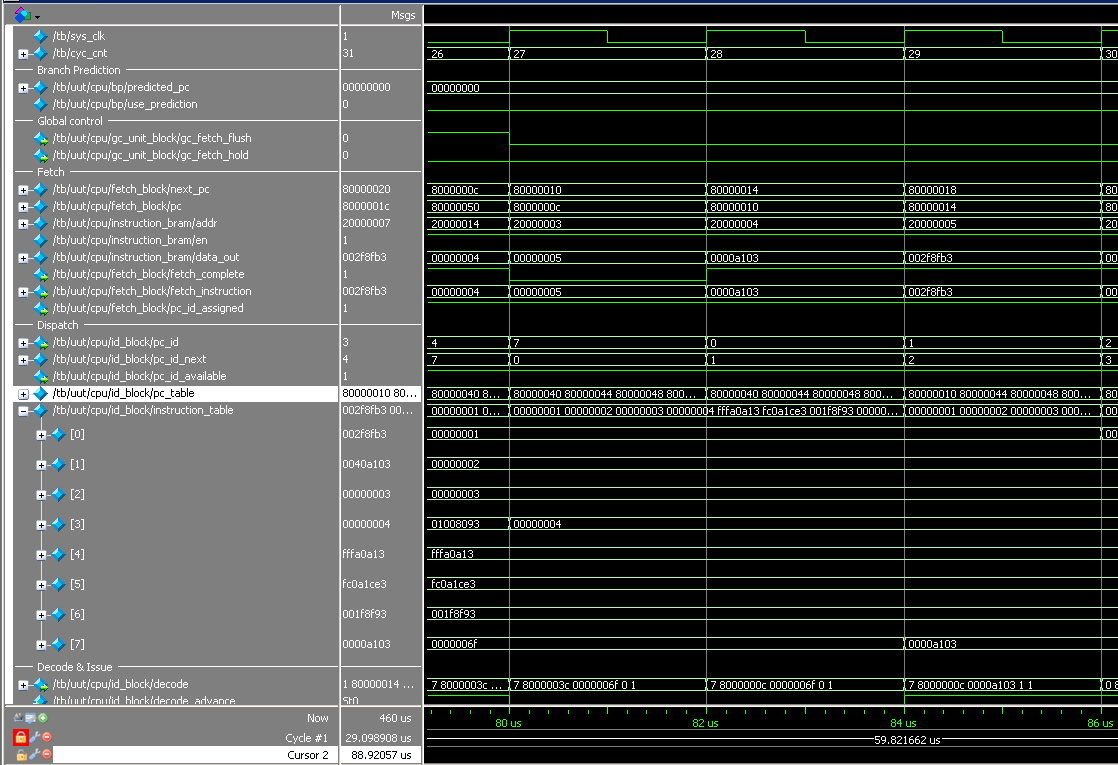
\includegraphics[scale=0.6]{assets/Task2.png}
	\end{center}
	\caption{Временная диаграмма выполнения стадий выборки и диспетчеризации команды 8000000c на 2-й итерации}
\end{figure}

\chapter{Задание №3}

На рисунке ниже рассмотренна временная диаграмма стадии декодирования и планирования на выполнение команды 80000018 на 2-й итерации цикла. В 34 такте происходит декодирование команды, в 35 она планируется на выполнение, возникает конфликт по регистру rs2, в 36 такте завершается выполнение предыдущей команды.

\begin{figure}[h!]
	\begin{center}
		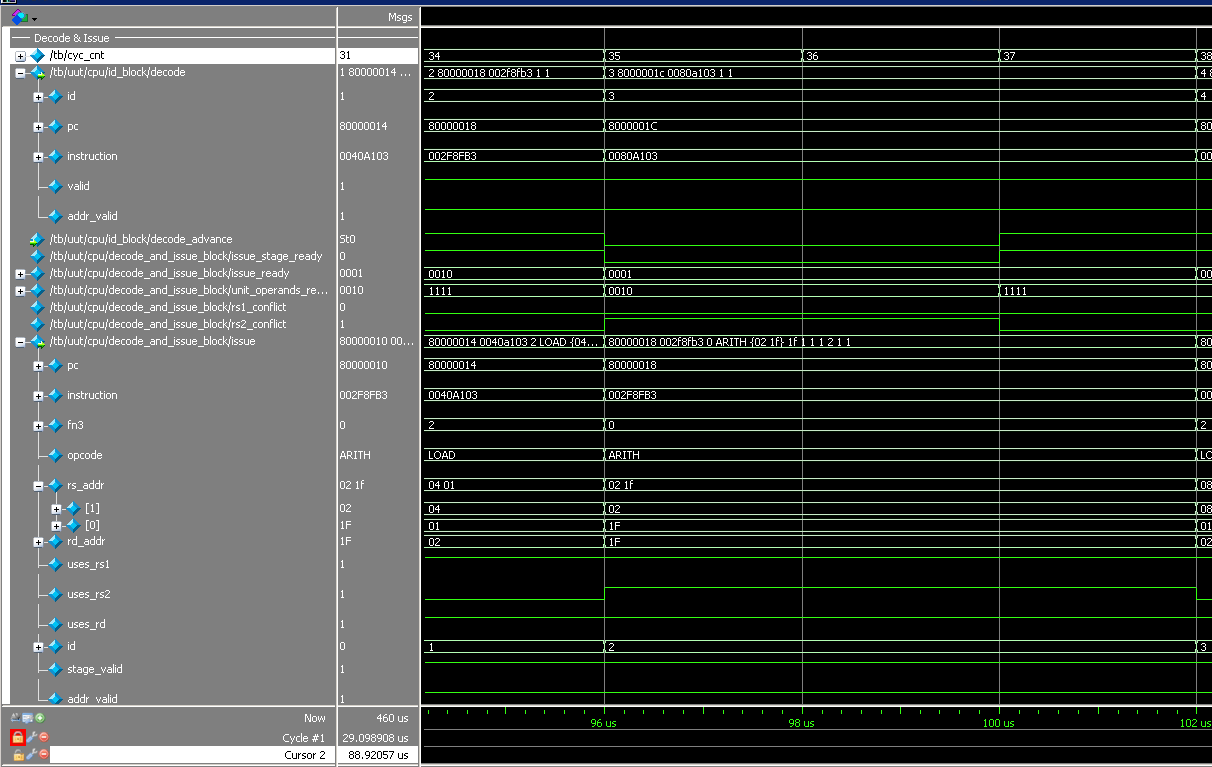
\includegraphics[scale=0.6]{assets/Task3.png}
	\end{center}
	\caption{Временная диаграмма выполнения стадий декодирования и планирования на выполнение команды 80000018 на 2-й итерации}
\end{figure}

\chapter{Задание №4}

На рисунке ниже рассмотренна временная диаграмма стадии выполнения команды 8000002c на 1-й итерации цикла. Видно, что в 23 такте данная команда поступает на выполнение, так как это арифметическая операция, она выполняется блоком ALU, в unit\_wb[0]/id записывается 3 (как и у исследуемой команды), сигнал unit\_wb[0]/done выставлен в 1. Следовательно выполнение данной команды завершается в этом же такте.

\begin{figure}[h!]
	\begin{center}
		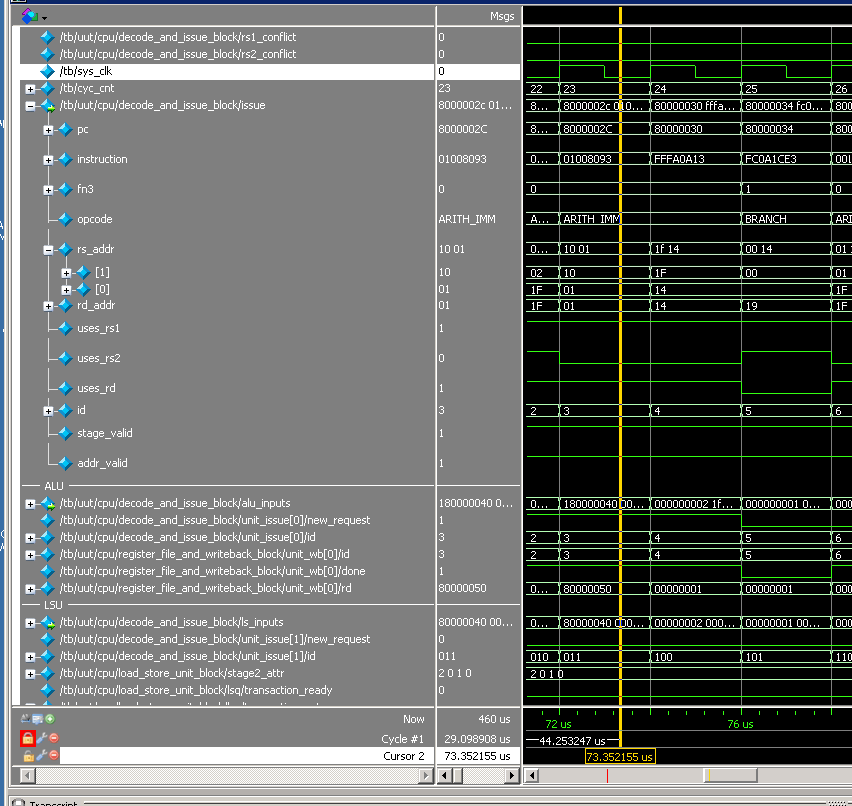
\includegraphics[scale=0.6]{assets/Task4.png}
	\end{center}
	\caption{Временная диаграмма выполнения стадии выполнения команды 8000002c на 1-й итерации}
\end{figure}

\chapter{Задание №5}

Для начала узнаем значение регистра $x31$, из рисунка ниже видно, что вычисленное в первом задании значение совпадает с хранящимся там
\begin{equation}
	00000025 (hex) = 37 (dec)
\end{equation}

\begin{figure}[h!]
	\begin{center}
		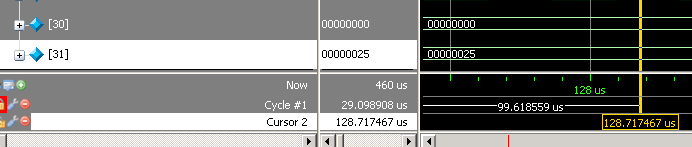
\includegraphics[scale=0.6]{assets/x31.png}
	\end{center}
	\caption{Значение регистра x31 после выполнения программы}
\end{figure}

Символом \#! в программе помечена команда addi x31, x31, x2. Рассмотрим стадии ее выполнения. На рисунке 5.1 представлены стадии выборки (6 такт), диспетчеризации (7 такт) и декодирования (8 такт).

\begin{figure}[h!]
	\begin{center}
		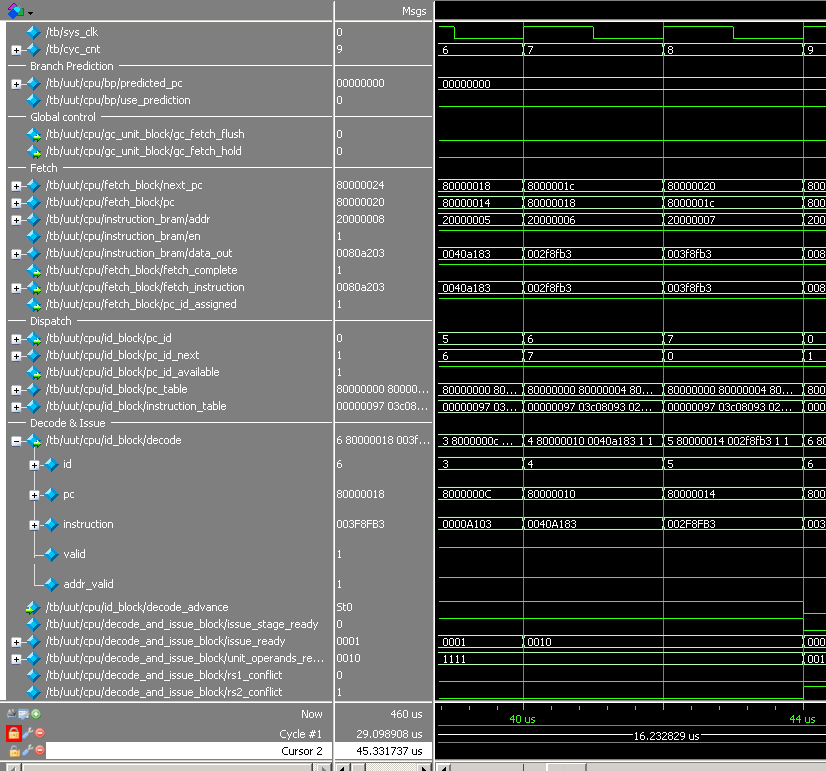
\includegraphics[scale=0.6]{assets/80000014.1.png}
	\end{center}
	\caption{Выборка, диспетчеризация и декодирование команды}
\end{figure}

В 9 такте команда планируется на выполнение, но так как сигнал rs2\_conflict равен 1 возникает конфликт. В следующем такте этот конфликт разрешается, управление передается блоку ALU, о чем свидетельтсвует совпадение issue/id и unit\_wb[0]/id, они равны 5. В 10 такте выполнение завершается, о чем свидетельствует 1 на сигнале unit\_wb[0]/done, и в следующем такте переходит к выполнению следующей команды.

\begin{figure}[h!]
	\begin{center}
		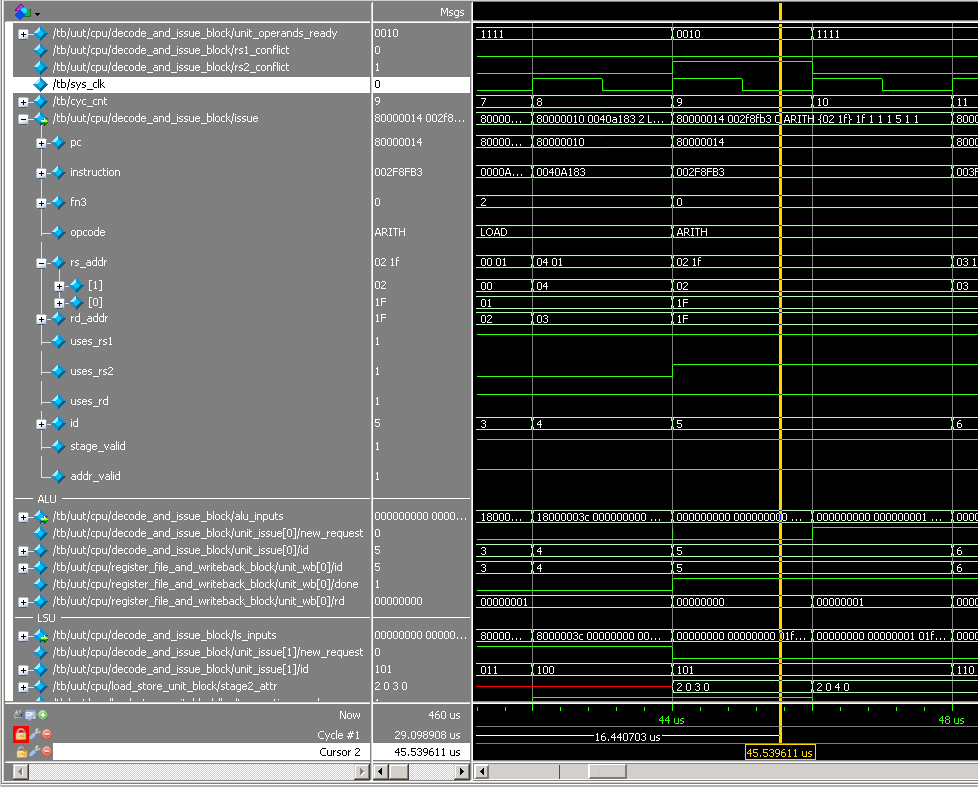
\includegraphics[scale=0.6]{assets/80000014.2.png}
	\end{center}
	\caption{Планирование на выполнение и выполнение команды}
\end{figure}

Ниже представленна временная диаграмма сигналов выполнения программы по варианту 12.
\newpage

\begin{figure}[h!]
	\begin{center}
		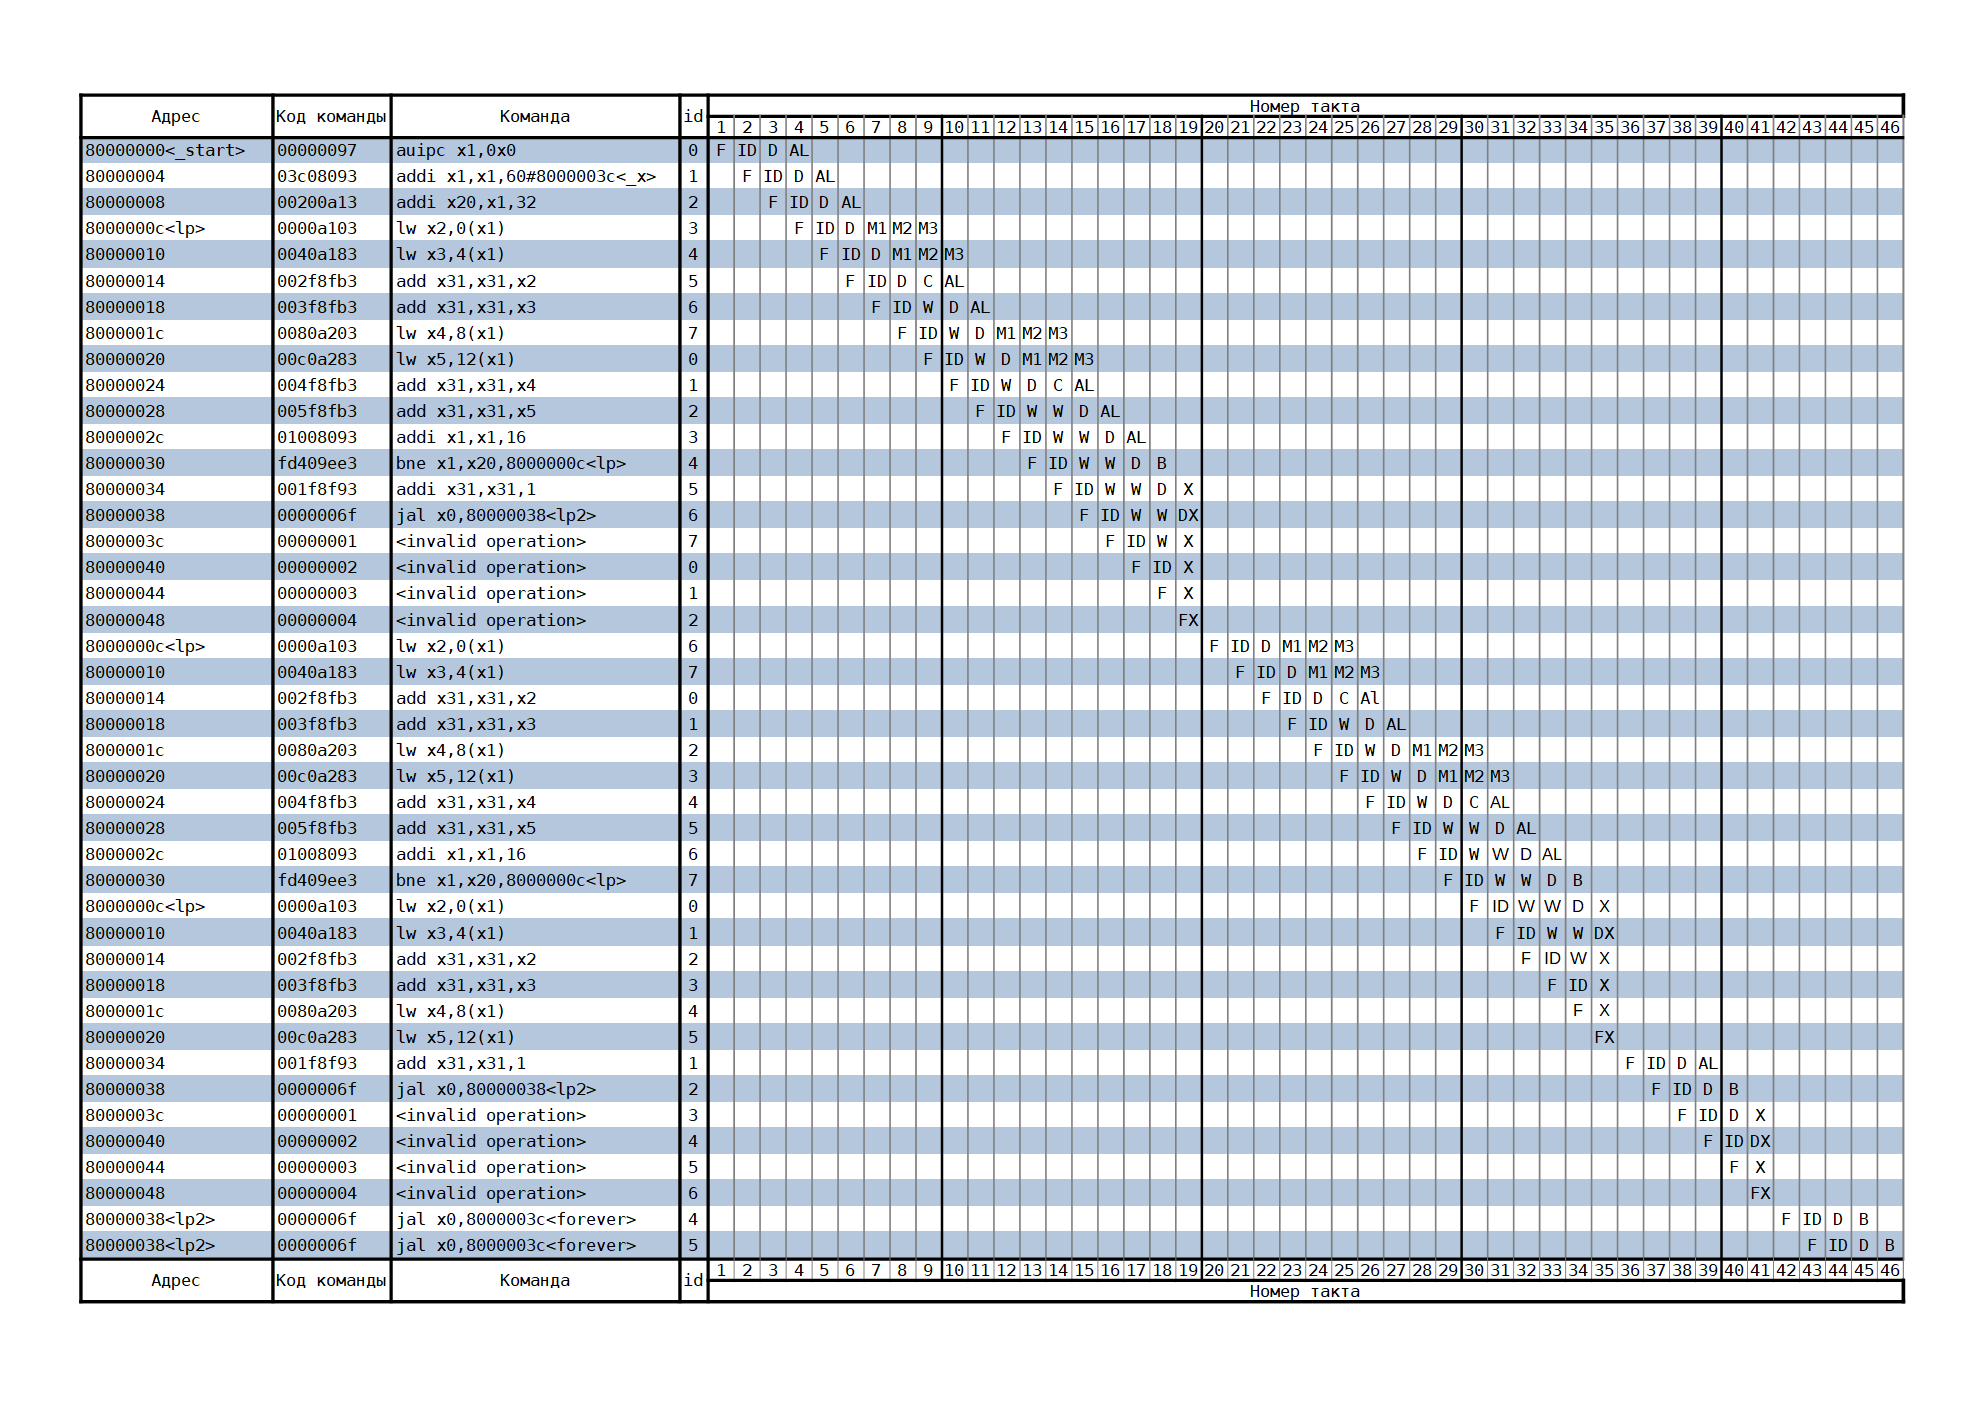
\includegraphics[scale=0.4]{assets/pipeline.png}
	\end{center}
	\caption{Временная диаграмма сигналов выполнения программы}
\end{figure}

Из трассы видно, что выполнение программы заканчивается выполнением команды add x31, x31, 1 в 39 такте. Тоесть выполнение программы происходит с 1 по 39 такт. Из них планирование на выполнение не происходило в течение 16 тактов (7, 8, 12, 13, 19 - 24, 28, 29, 35 - 38). Это составляет 41\%. Чтобы сократить время простоя можно провести оптимизацию путем перестановки команд. 

В качестве оптимизации было выбрано перемещение строк загрузки данных друг к другу. Оптимизированный код представлен на листинге ниже.

\newpage
\begin{lstlisting}[label=code, caption=Код оптимизированной программы]
  .section .text
        .globl _start;
        len = 8 #array length
        enroll = 4 #count of elems in one loop
		elem_sz = 4 #size of one element

_start:
        la x1, _x
        addi x20, x1, elem_sz*len #address of last elem
lp:
        lw x2, 0(x1)
        lw x3, 4(x1)
        lw x4, 8(x1)
        lw x5, 12(x1)
        add x31, x31, x2 #!
        add x31, x31, x3
        add x31, x31, x4
        add x31, x31, x5
        addi x1, x1, elem_sz*enroll
        bne x1, x20, lp
        addi x31, x31, 1
lp2: j lp2

        .section .data
_x:     .4byte 0x1
        .4byte 0x2
        .4byte 0x3
        .4byte 0x4
        .4byte 0x5
        .4byte 0x6
        .4byte 0x7
        .4byte 0x8
\end{lstlisting}
\newpage

Временная диаграмма сигналов выполнения представленна ниже.

\begin{figure}[h!]
	\begin{center}
		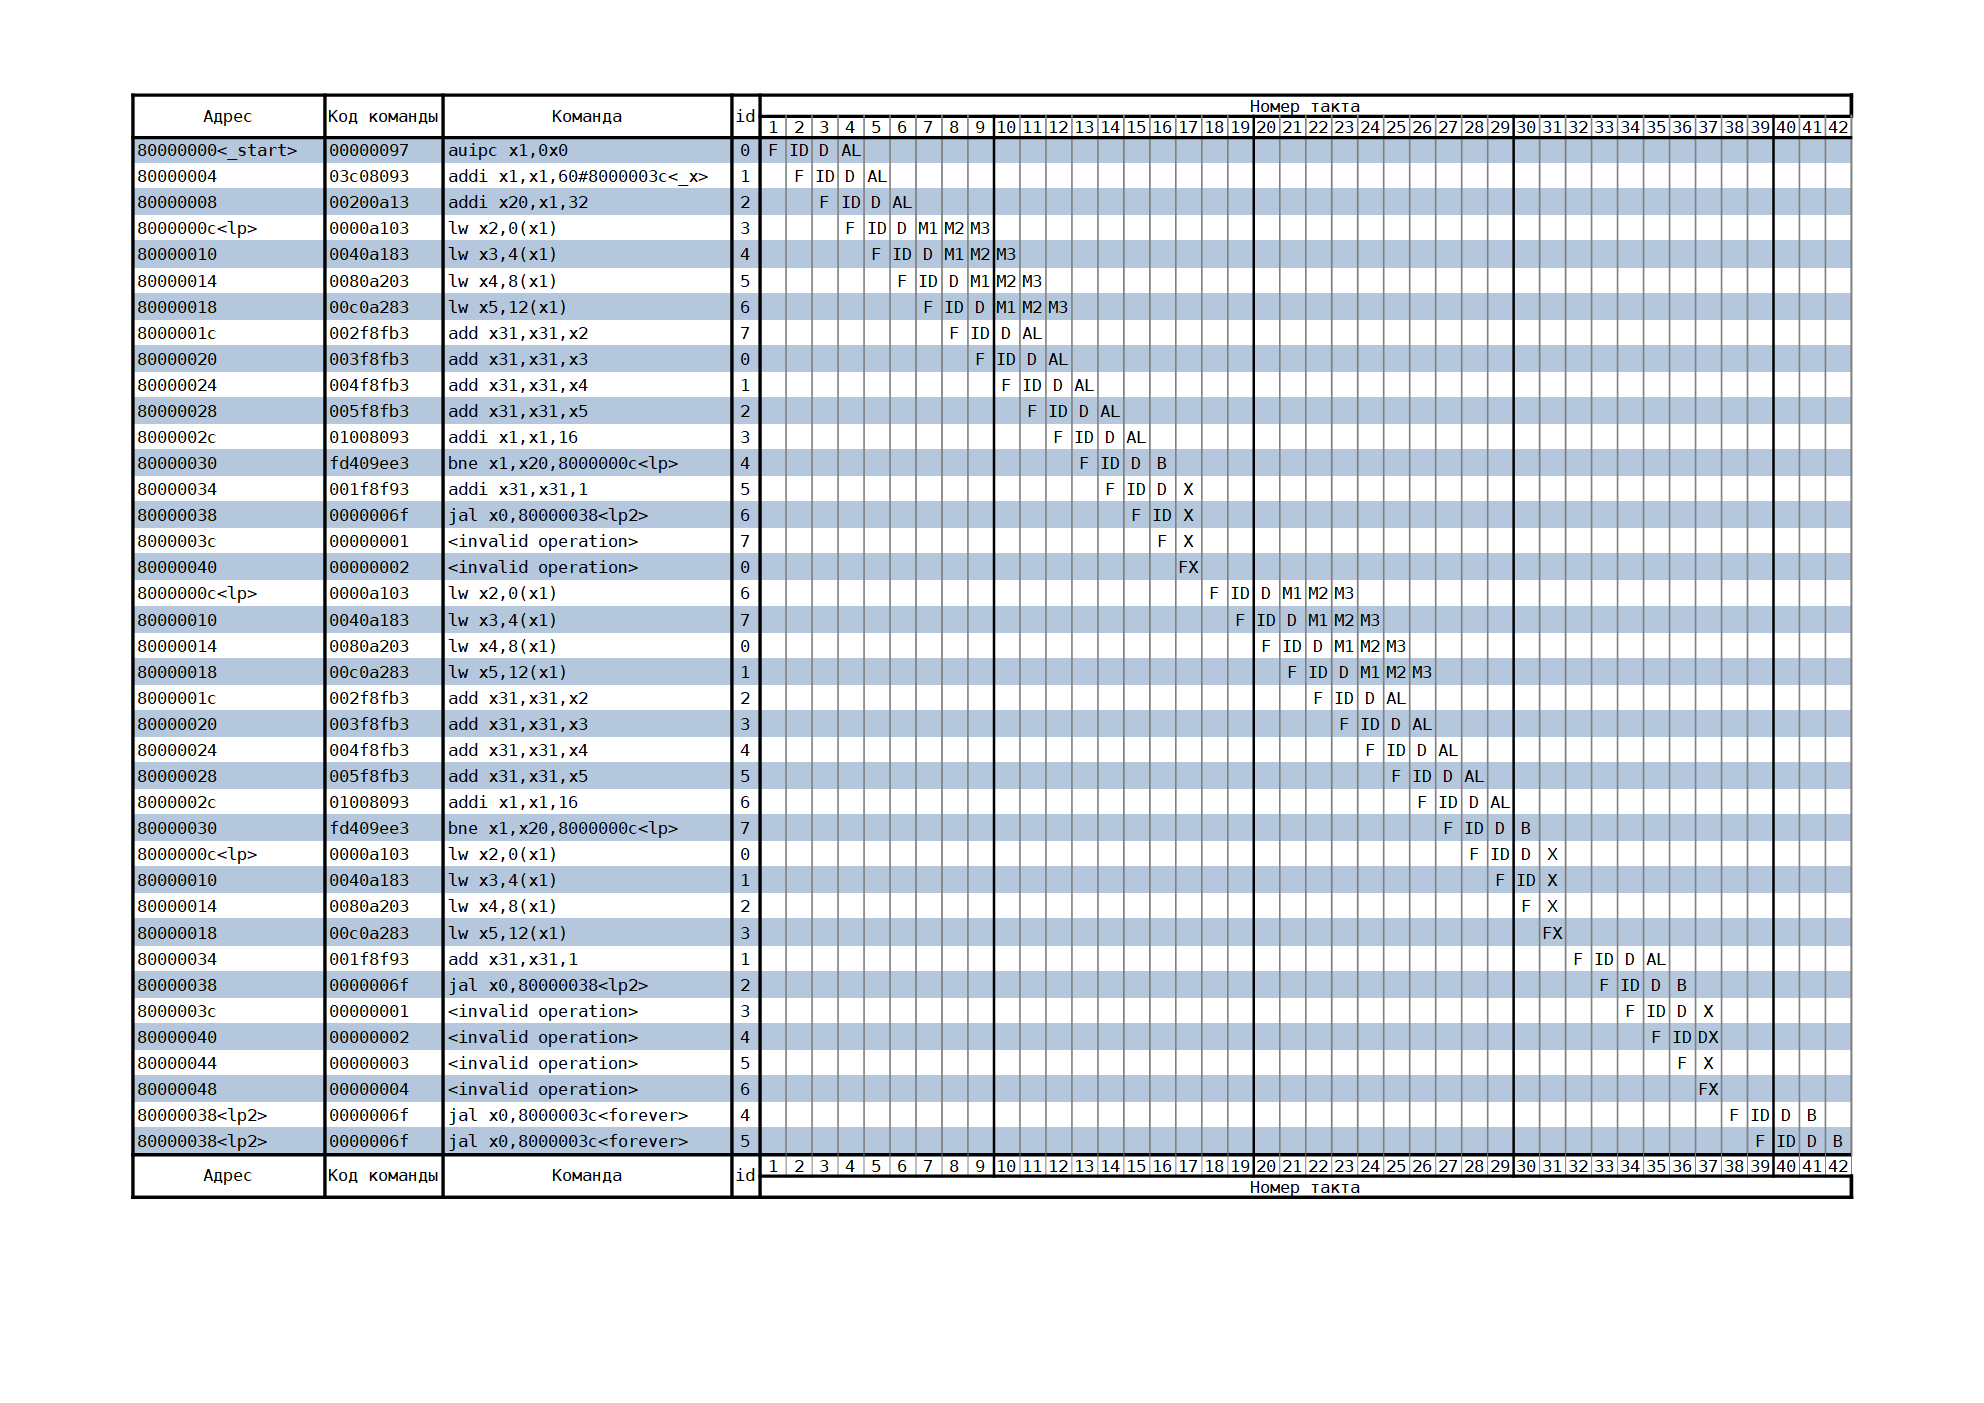
\includegraphics[scale=0.4]{assets/pipelineOpt.png}
	\end{center}
	\caption{Временная диаграмма сигналов выполнения оптимизированной программы}
\end{figure}

Из трассы видно, что выполнение программы заканчивается выполнением команды add x31, x31, 1 в 35 такте. Тоесть выполнение программы происходит с 1 по 35 такт. Из них планирование на выполнение не происходило в течение 12 тактов (7, 8, 17 - 22, 31 - 34). Это составляет 31\%. Удалось сократить простой на 10\%.